\documentclass[32pt,portrait]{tikzposter}
\geometry{paperwidth=30in,paperheight=40in,width=28in,height=38in}
%\trimFrame
%\settrimmedsize{1in}{1in}{*}
%\settrims{20mm}{34mm}
%\usepackage{beamer}
%\usepackage[paperwidth=30in,paperheight=40in,margin=1in]{beamerposter}
\usepackage{graphicx}
\usepackage{eso-pic,xcolor}
\usepackage{float}
\usepackage{color}
\usepackage{tikz}
\usepackage{subfig}
\usepackage{verbatim}
\title{Membership survey of the Alpha Persei open stellar cluster}
\author{Graham Roberts, Kevin Covey}
\institute{Western Washington University}
\setlength{\fboxsep}{0in}%
\setlength{\fboxrule}{0.375in}%
\definecolorstyle{sw16}{
	\definecolor{orchid}{RGB}{249,38,114}
	\definecolor{PumpkinSpice}{RGB}{253,151,31}
	\definecolor{sundriedClay}{RGB}{39,40,34}
	\definecolor{bg}{RGB}{230,230,250}
	\definecolor{violetBorder}{RGB}{98,22,141}
	\definecolor{bounded rationality}{RGB}{102,217,239}
}{
\colorlet{backgroundcolor}{sundriedClay}
\colorlet{framecolor}{violetBorder}
\colorlet{titlefgcolor}{bounded rationality}
\colorlet{titlebgcolor}{black}
\colorlet{blocktitlebgcolor}{black}
\colorlet{blocktitlefgcolor}{orchid}
\colorlet{blockbodybgcolor}{bg}
\colorlet{blockbodyfgcolor}{sundriedClay}
\colorlet{innerblocktitlebgcolor}{black}
\colorlet{innerblocktitlefgcolor}{orchid}
\colorlet{innerblockbodybgcolor}{bg}
\colorlet{innerblockbodyfgcolor}{black}
}
\defineblockstyle{sampleblockstyle}{
titlewidthscale=0.9, bodywidthscale=1,titleleft,
titleoffsetx=0pt, titleoffsety=0pt, bodyoffsetx=0mm, bodyoffsety=15mm,
bodyverticalshift=10mm, roundedcorners=5, linewidth=2pt,
titleinnersep=6mm, bodyinnersep=1cm
}{
\draw[color=blockbodyfgcolor, fill=blockbodybgcolor,
rounded corners=\blockroundedcorners] (blockbody.south west)
rectangle (blockbody.north east);
\ifBlockHasTitle
\draw[color=blocktitlefgcolor, fill=blocktitlebgcolor,
rounded corners=\blockroundedcorners] (blocktitle.south west)
rectangle (blocktitle.north east);
\fi
}

\definetitlestyle{apsw}{
	width=28in, roundedcorners=5, linewidth=2pt, innersep=5pt,titletotopverticalspace=0.25in}
{\begin{scope}[line width=\titlelinewidth, rounded corners=\titleroundedcorners]
	\draw[color=titlefgcolor, fill=titlebgcolor]
		(\titleposleft,\titleposbottom) rectangle (\titleposright, \titlepostop);
	\end{scope}
}
%\usepackage{wallpaper}
\usecolorstyle{sw16}
\usetitlestyle{apsw}
\useblockstyle{sampleblockstyle}
\begin{document}
\maketitle
\begin{centering}
\begin{columns}

%\begin{tikzfigure}[3d plot of membersip probabilities over geomwtric distance and proper motion distance]
%\begin{tikzpicture}
%\includegraphics{poster3dalpha};
%\end{tikzpicture}
%\end{tikzfigure}}
\column{.4}
\block[bodywidthscale=.85,bodyoffsetx=.9in,titleoffsetx=.8in, bodyoffsety=1.1in,titleoffsety=.7in]{Introduction}{\begin{itemize}
\item Alpha Persei ($\alpha$ Per) is a young Stellar Open Cluster.
\item Open clusters are groups of stars that formed at the same time from the same interstellar molecular cloud.
\item Cluster ages can be determined by fitting stellar evolution models to the measured properties of cluster's evolved stars.
\item These are used to calibrate measurements of other stellar properties. 
\item $\alpha$ Per is relatively close which gives it large proper motion, or movement relative to other stars in the plane of the sky.
\item We can use these measurements of position and proper motion to identify other members of $\alpha$ Per.
\item We need to identify more members in order to better determine the age of the custer.
\end{itemize}}
%\block[bodyoffsetx=1.2in,titleoffsetx=1.2in]{Abstract}{Alpha Persei is a young stellar open cluster in our Galaxy.  Stellar open clusters are groups of stars that formed at the same time from a single cloud in the interstellar medium.  Cluster's well defined ages allow astronomers to calibrate stellar evolution models with measurements of constituent members, and track the history of star formation in the Milky Way.  Alpha Persei is relatively young, on the scale of around 100 million years old (Shiekhi et al. 2016).  Alpha Per provides a key laboratory for studying the properties, such as mass, radii, temperature, etc. of young stars.  We have yet to identify enough members of the cluster to more accurately estimate its age.  This is why a membership survey is important.  Since stellar clusters form close together the members interact gravitationally resulting in a mass of stars that are very close together.  More interestingly they all move at nearly the same velocity through the Galaxy. Alpha Per's proximity is such that the cluster's velocity through space produces a large proper motion, or apparent angular momentum in the plane of the sky, relative to other stars in our Galaxy.  We model the cluster population of stars using each star's position in the night sky as well as proper motion. Analyzing these distributions we reduce a database down to a manageable number of stars that are  probably also members of the cluster, down to under 100,000 from 4 million.  This membership catalogue will allow us to complete a more precise study of the cluster's age.}
%[bodyoffsety=.5in, titleoffsety=.5in,bodyoffsetx=-.8in, ,titleoffsetx=-.9in, bodywidthscale=1]
\column{.1}
\column{.4}
\block[bodyoffsety=.7in,titleoffsety=.7in]{Membership Probability}{
\begin{tikzfigure}[Scatter plot of projected membership probabilities for field stars near the $\alpha$ Per open cluster. The x-axis shows their radial distance from the cluster center and the y-axis illustrates the difference between the cluster's mean in proper motion and that of the candidate members.]
 %     \begin{tikzpicture}
   %   \begin{centering}
      \includegraphics[scale=.8]{poster3dresize}
  %    \end{centering}
  %    \end{tikzpicture}
      \end{tikzfigure}
}
\column{.1}
\end{columns}
%\block[bodywidthscale=.9]{Alpha Persei}{As mentioned the Alpha Persei cluster is a group of nearby young stars.  This cluster is relatively well spread out compared to other star clusters.  Previous Surveys identified many members, however not enough to get a terribly accurate age estimate.  Our method for performing this age estimate is by fitting a model isochrone the the color and magnitude of the cluster.  The current Membership survey of $\alpha$ per unfortunately lacking in stars who's color and magnitude fall around the turnoff on the color magnitude diagram. This is unfortunately the point at which these model diverge the most with age.  For that reason our study has thus far focused on a membership survey.}
\begin{columns}
\column{.4}

\begin{subcolumns}
\subcolumn{.45}
\block[bodywidthscale=1.1,bodyoffsetx=1.6in,titleoffsetx=1.325in, bodyoffsety=1.5in, titleoffsety=.5in]{Spatial Distribution}{
\begin{tikzfigure}[Spatial distribution in right ascension and declination of catalog stars and known members, see symbols from Fig. 1.  Cluster members show some preference towards center, howerver field stars are for the most part uniform.]
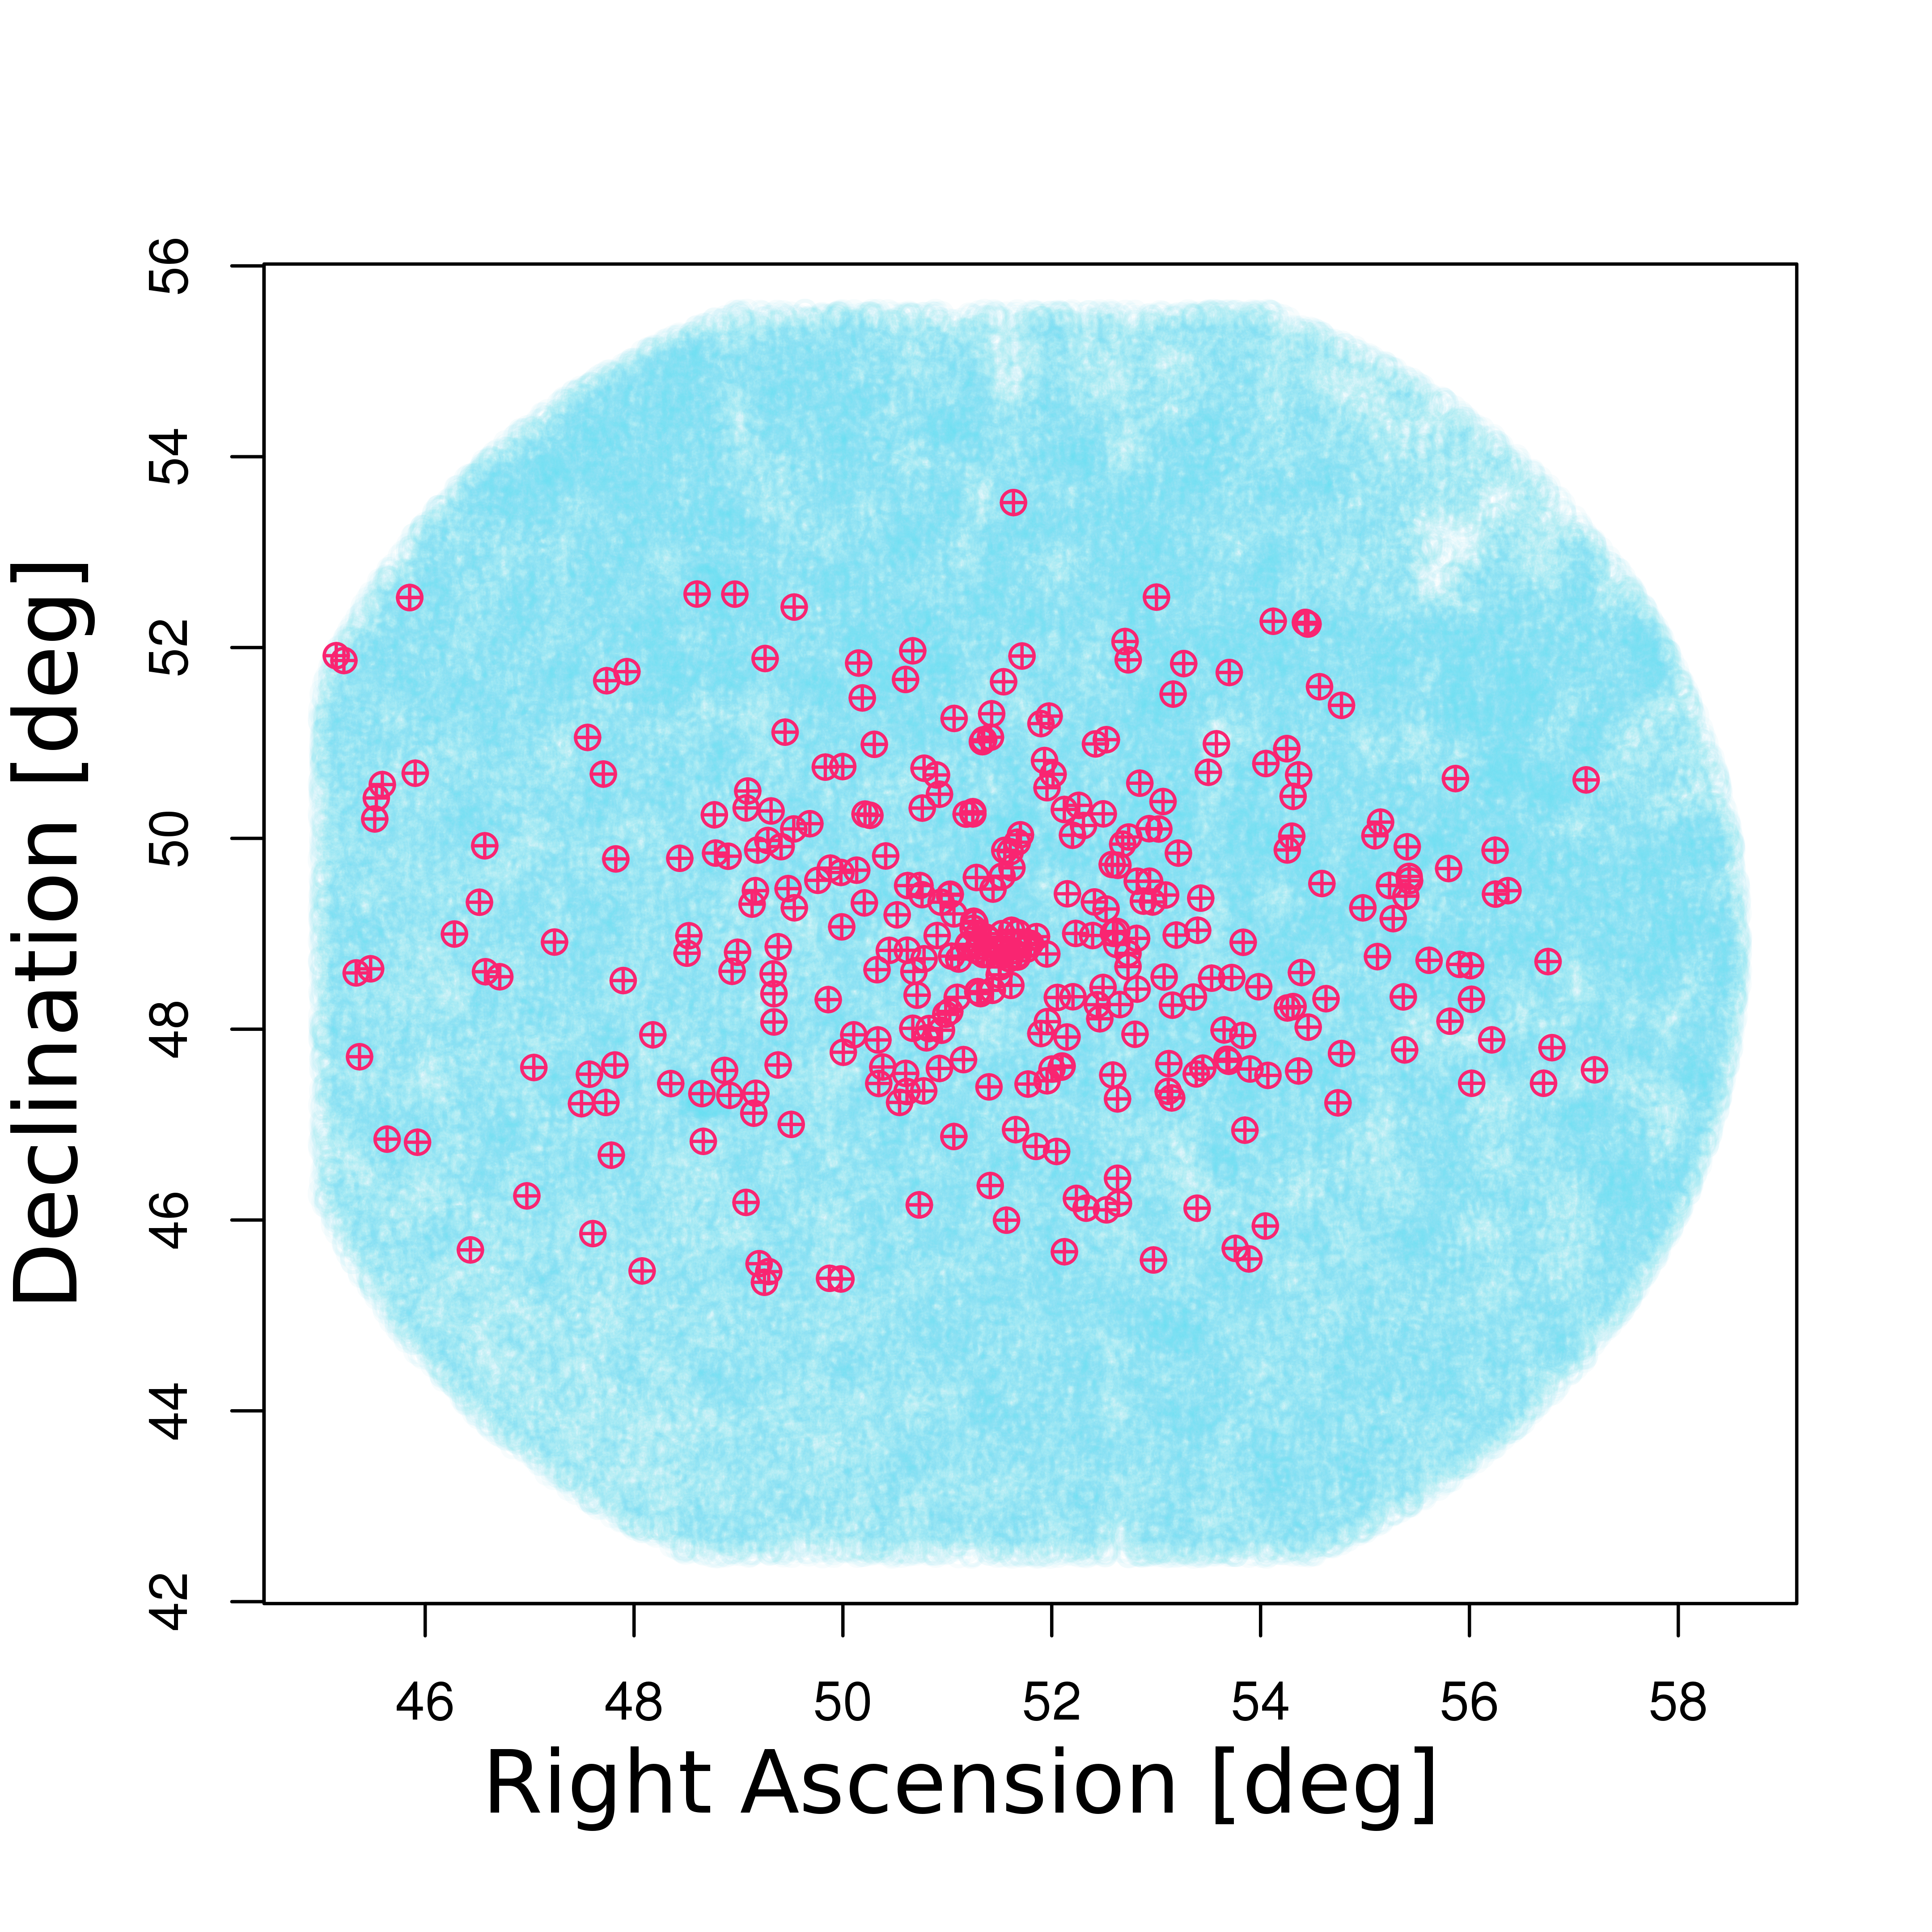
\includegraphics[scale=.9]{SpaDis2}
%\end{center}
\end{tikzfigure}
}
\block[bodywidthscale=1.1,bodyoffsetx=1.6in,titleoffsetx=1.325in, bodyoffsety=1.5in, titleoffsety=.5in]{Proper Motion Distribution}{
\begin{tikzfigure}[distribution in proper motion right ascension and proper motion declination. Member stars heavily localized, while field stars heavily localized elsewhere]
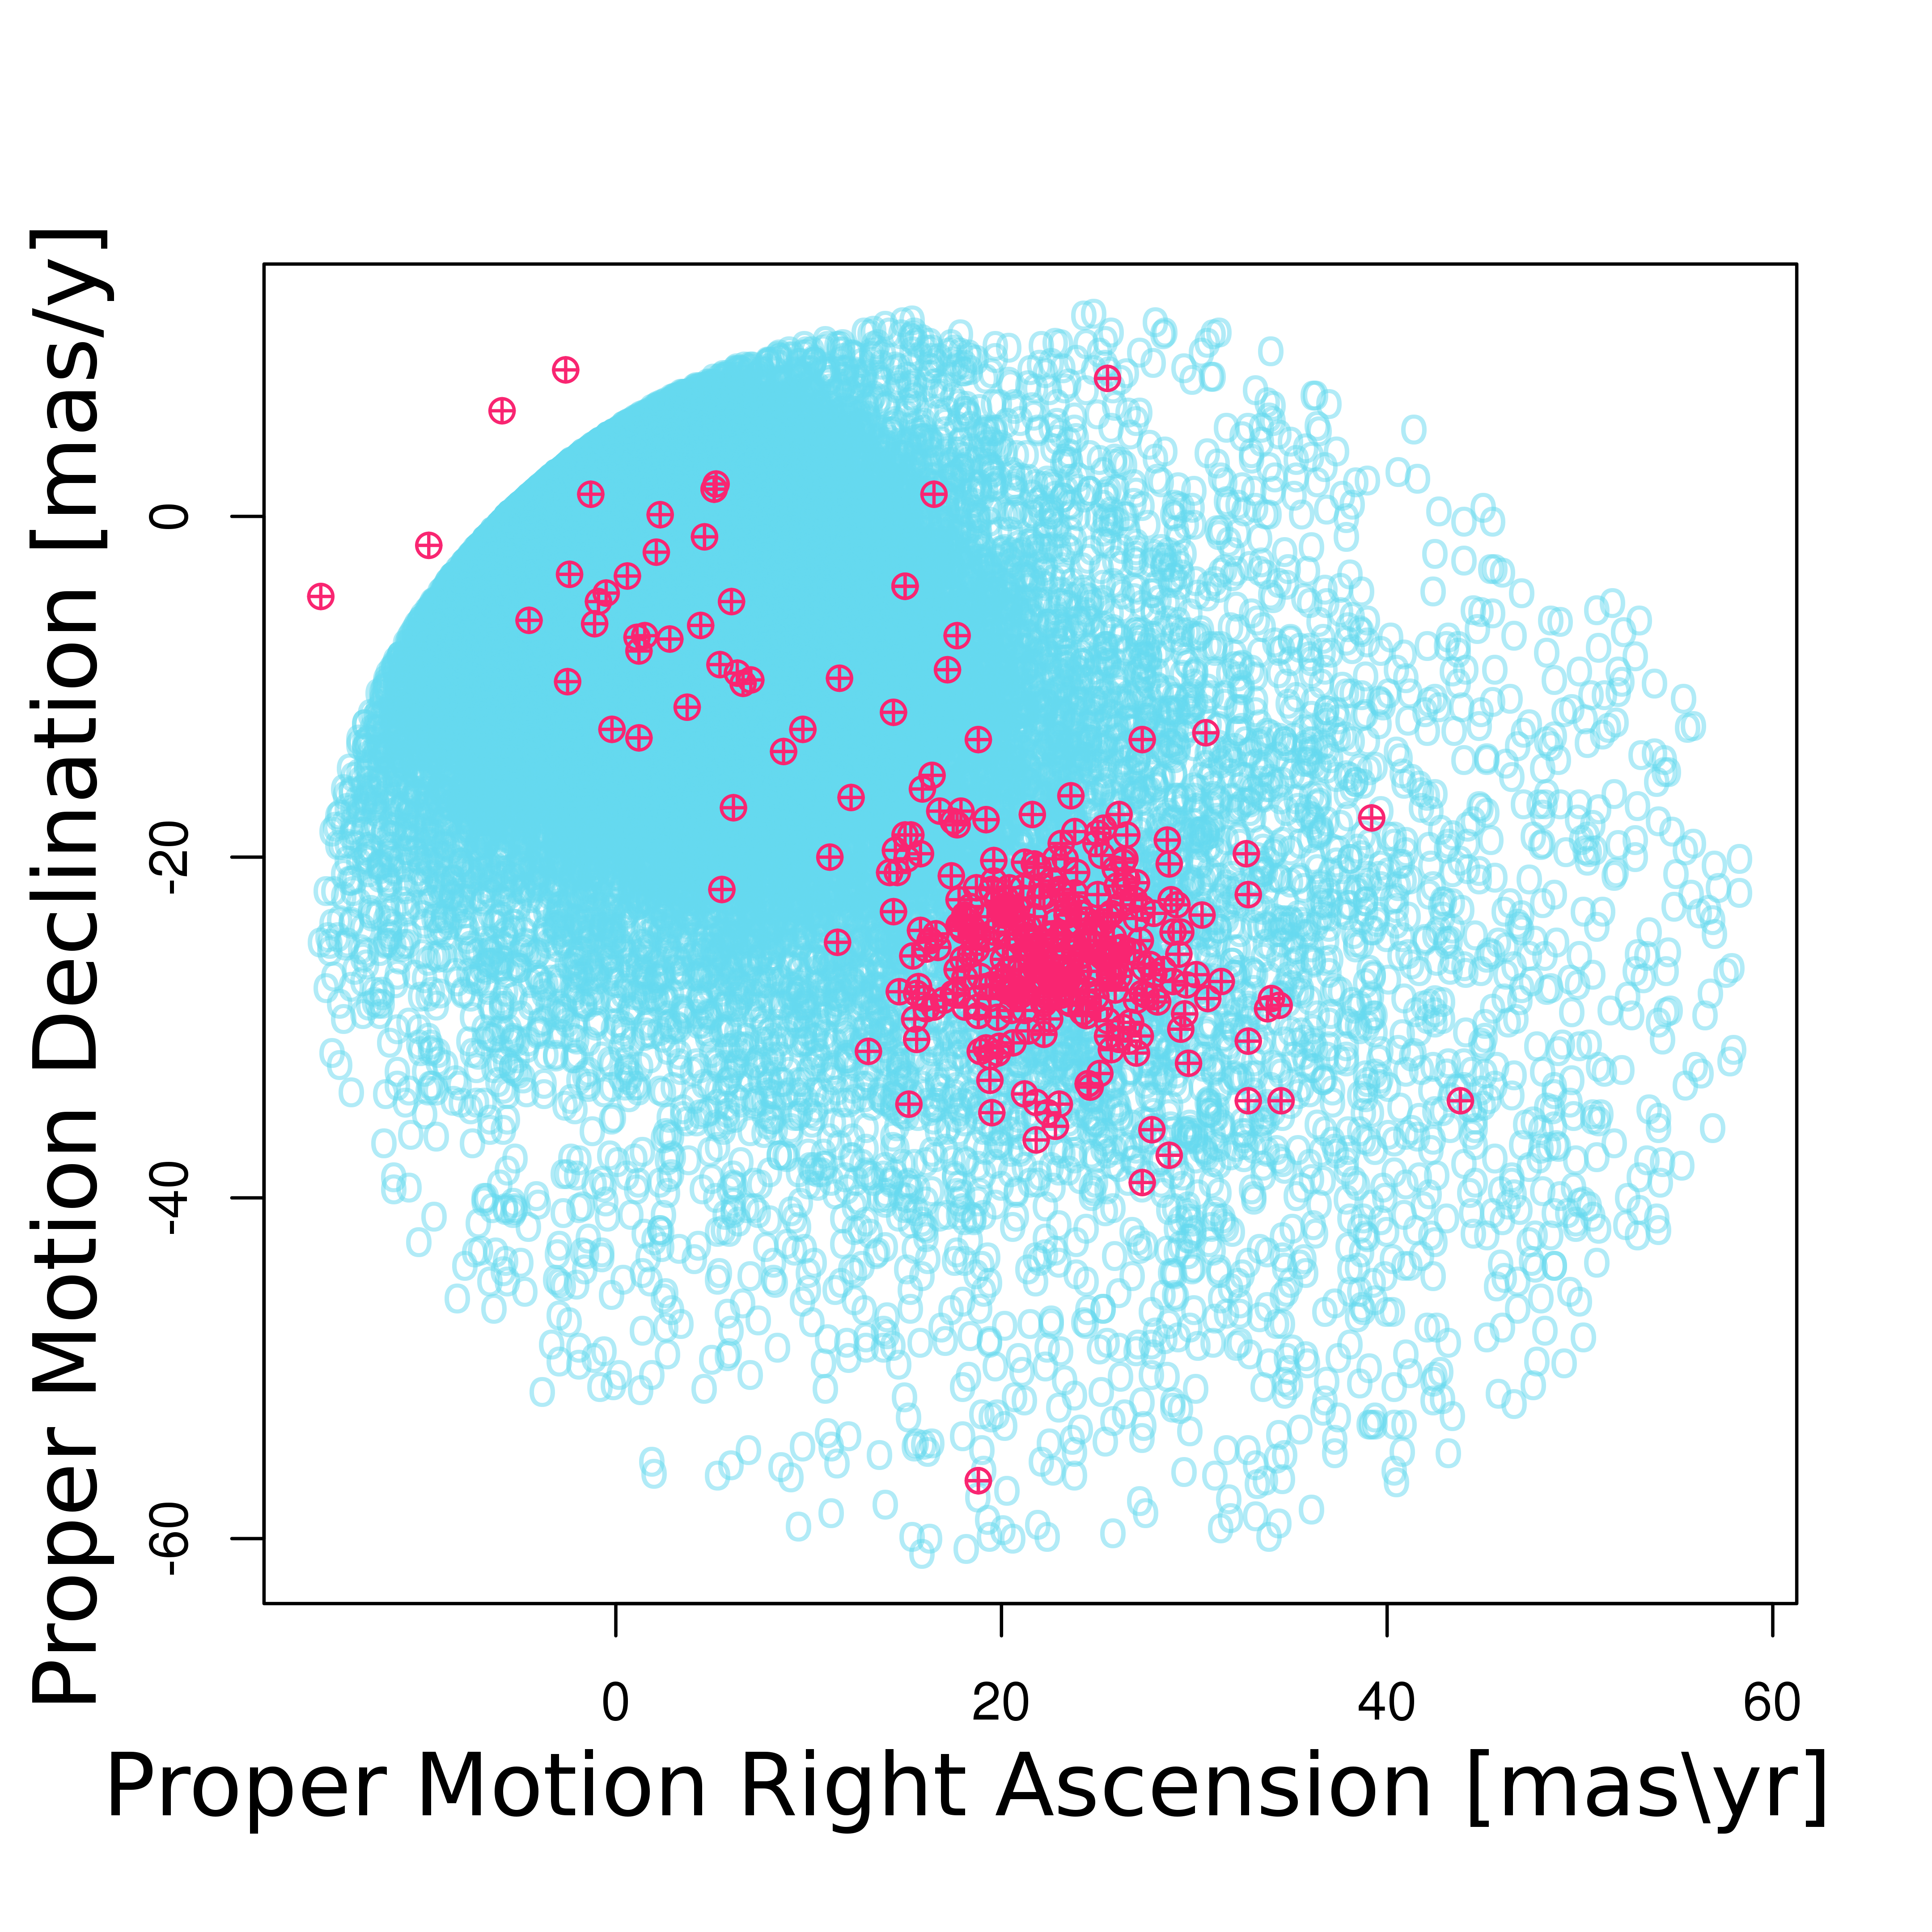
\includegraphics[scale=.9]{ProDis}
%\end{center}
\end{tikzfigure}

}
\subcolumn{.45}
\block[bodywidthscale=1.2,bodyoffsetx=1.7in,titleoffsetx=1.55in,bodyoffsety=1.7in, titleoffsety=.5in]{Spatial Probability}{
\begin{tikzfigure}[Membership Probability over radial distance. Members show high probability at their distances relative to the catalog stars, due to high proper motion probability.]
\includegraphics[scale=.9]{SpaPro}
\end{tikzfigure}

}
\block[bodywidthscale=1.2,bodyoffsetx=1.7in,titleoffsetx=1.55in,bodyoffsety=1.7in,titleoffsety=.5in]{Proper Motion Probability}{
\begin{tikzfigure}[Membership Probability over proper motion distance.  Member stars localized at low differences from the mean proper motion.]
\includegraphics[scale=.9]{ProPro}
\end{tikzfigure}
}

\end{subcolumns}

\column{.55}

\block[bodywidthscale=.9,bodyoffsetx=1in,titleoffsetx=1.25in,titlewidthscale=.65,bodyoffsety=1in,titleoffsety=.5in]{Selection Methods}{
\begin{itemize}
\item Cluster properties (mean proper motion, central position, etc.) adopted from previous surveys[1-3] to determine membership.
\item We used Data for field stars within a small rectangle centered on $\alpha$ Per, taken from the URAT1 catlog.
\item The spatial distribution of known members is densest towards the cluster center, but exhibits a considerable spread [see Fig. 2 \& 4]. Field stars in the same region are distributed relatively uniformly on the sky, however.
\item URAT catalog includes $\approx$700 more stars in this region than expected based on extrapolating the uniform distribution of field stars accross the whole region; we adopt this estimate of $\approx700$ total cluster members to calculate the membership probability $P(M)$ for each star in this region.
\item Members of $\alpha$ Per have high proper motion due to the cluster's proximity, which produces large angular velocities.
\item More distant field stars tend to have much smaller proper motion than members.
\item We modeled the probability of a star being a certain distance from the cluster mean in position or proper motion given membership, $P(R|M)$, from previous members.
\item We calculated the probability of being a distance from the mean, $P(R)$.
\item We calculate the probability of being a member given a certain difference from the mean in either position or proper motion using Bayes' Theorem:
\begin{equation}
P(M|R)=\frac{P(R|M)P(M)}{P(R)}
\end{equation}
[see Fig. 4 \& 5].
\item We still need to acquire data on the parallax of member stars and determine their spatial distribution in three dimensions including distance.
\item We will then calulate a model of the light emitted by these stars, and find an age that would produce an isochrone that best matched.
\end{itemize}}
\block[bodyoffsetx=1in,titleoffsetx=1in,bodywidthscale=.9, titleoffsety=.5in, bodyoffsety=1in]{References}{
\begin{enumerate}
\item Deacon, N. R., Hambly, N. C. (2004). ``Proper motion surveys of the young open clusters Alpha Persei and the Pleiades" \textit{Astronomy and Astrophysics}. Vol 416. 125-136.
\item Prosser, Charles, F. (1992, February). ``Membership of low-mass stars in the open cluster $\alpha$ Persei"  \textit{The Astronomical Journal}. Vol. 103(2), 488-513. 
\item Shiekhi, N., Hasheminia, M., Khalaj, P., Haghi, H., Hasani Zoonozi, A., Baumgardt, H. (28 July 2015) ``The binary fraction and mass segregation in Alpha Persei open cluster" \textit{Monthly Notices of the Royal Astronomy Society}. Vol. 457, 1028-1036.
\end{enumerate}
}
%\column{.4}
%\begin{subcolumns}
%\subcolumn{.45}
%\block[bodywidthscale=1.2,bodyoffsetx=.3in,titleoffsetx=.225in, bodyoffsety=1in, titleoffsety=.5in]{Spatial Distribution}{
%\begin{tikzfigure}[Spatial distribution in right ascension and declination of catalog stars and known members, see symbols from Fig. 1.  Cluster members show some preference towards center, howerver field stars are for the most part uniform.]
%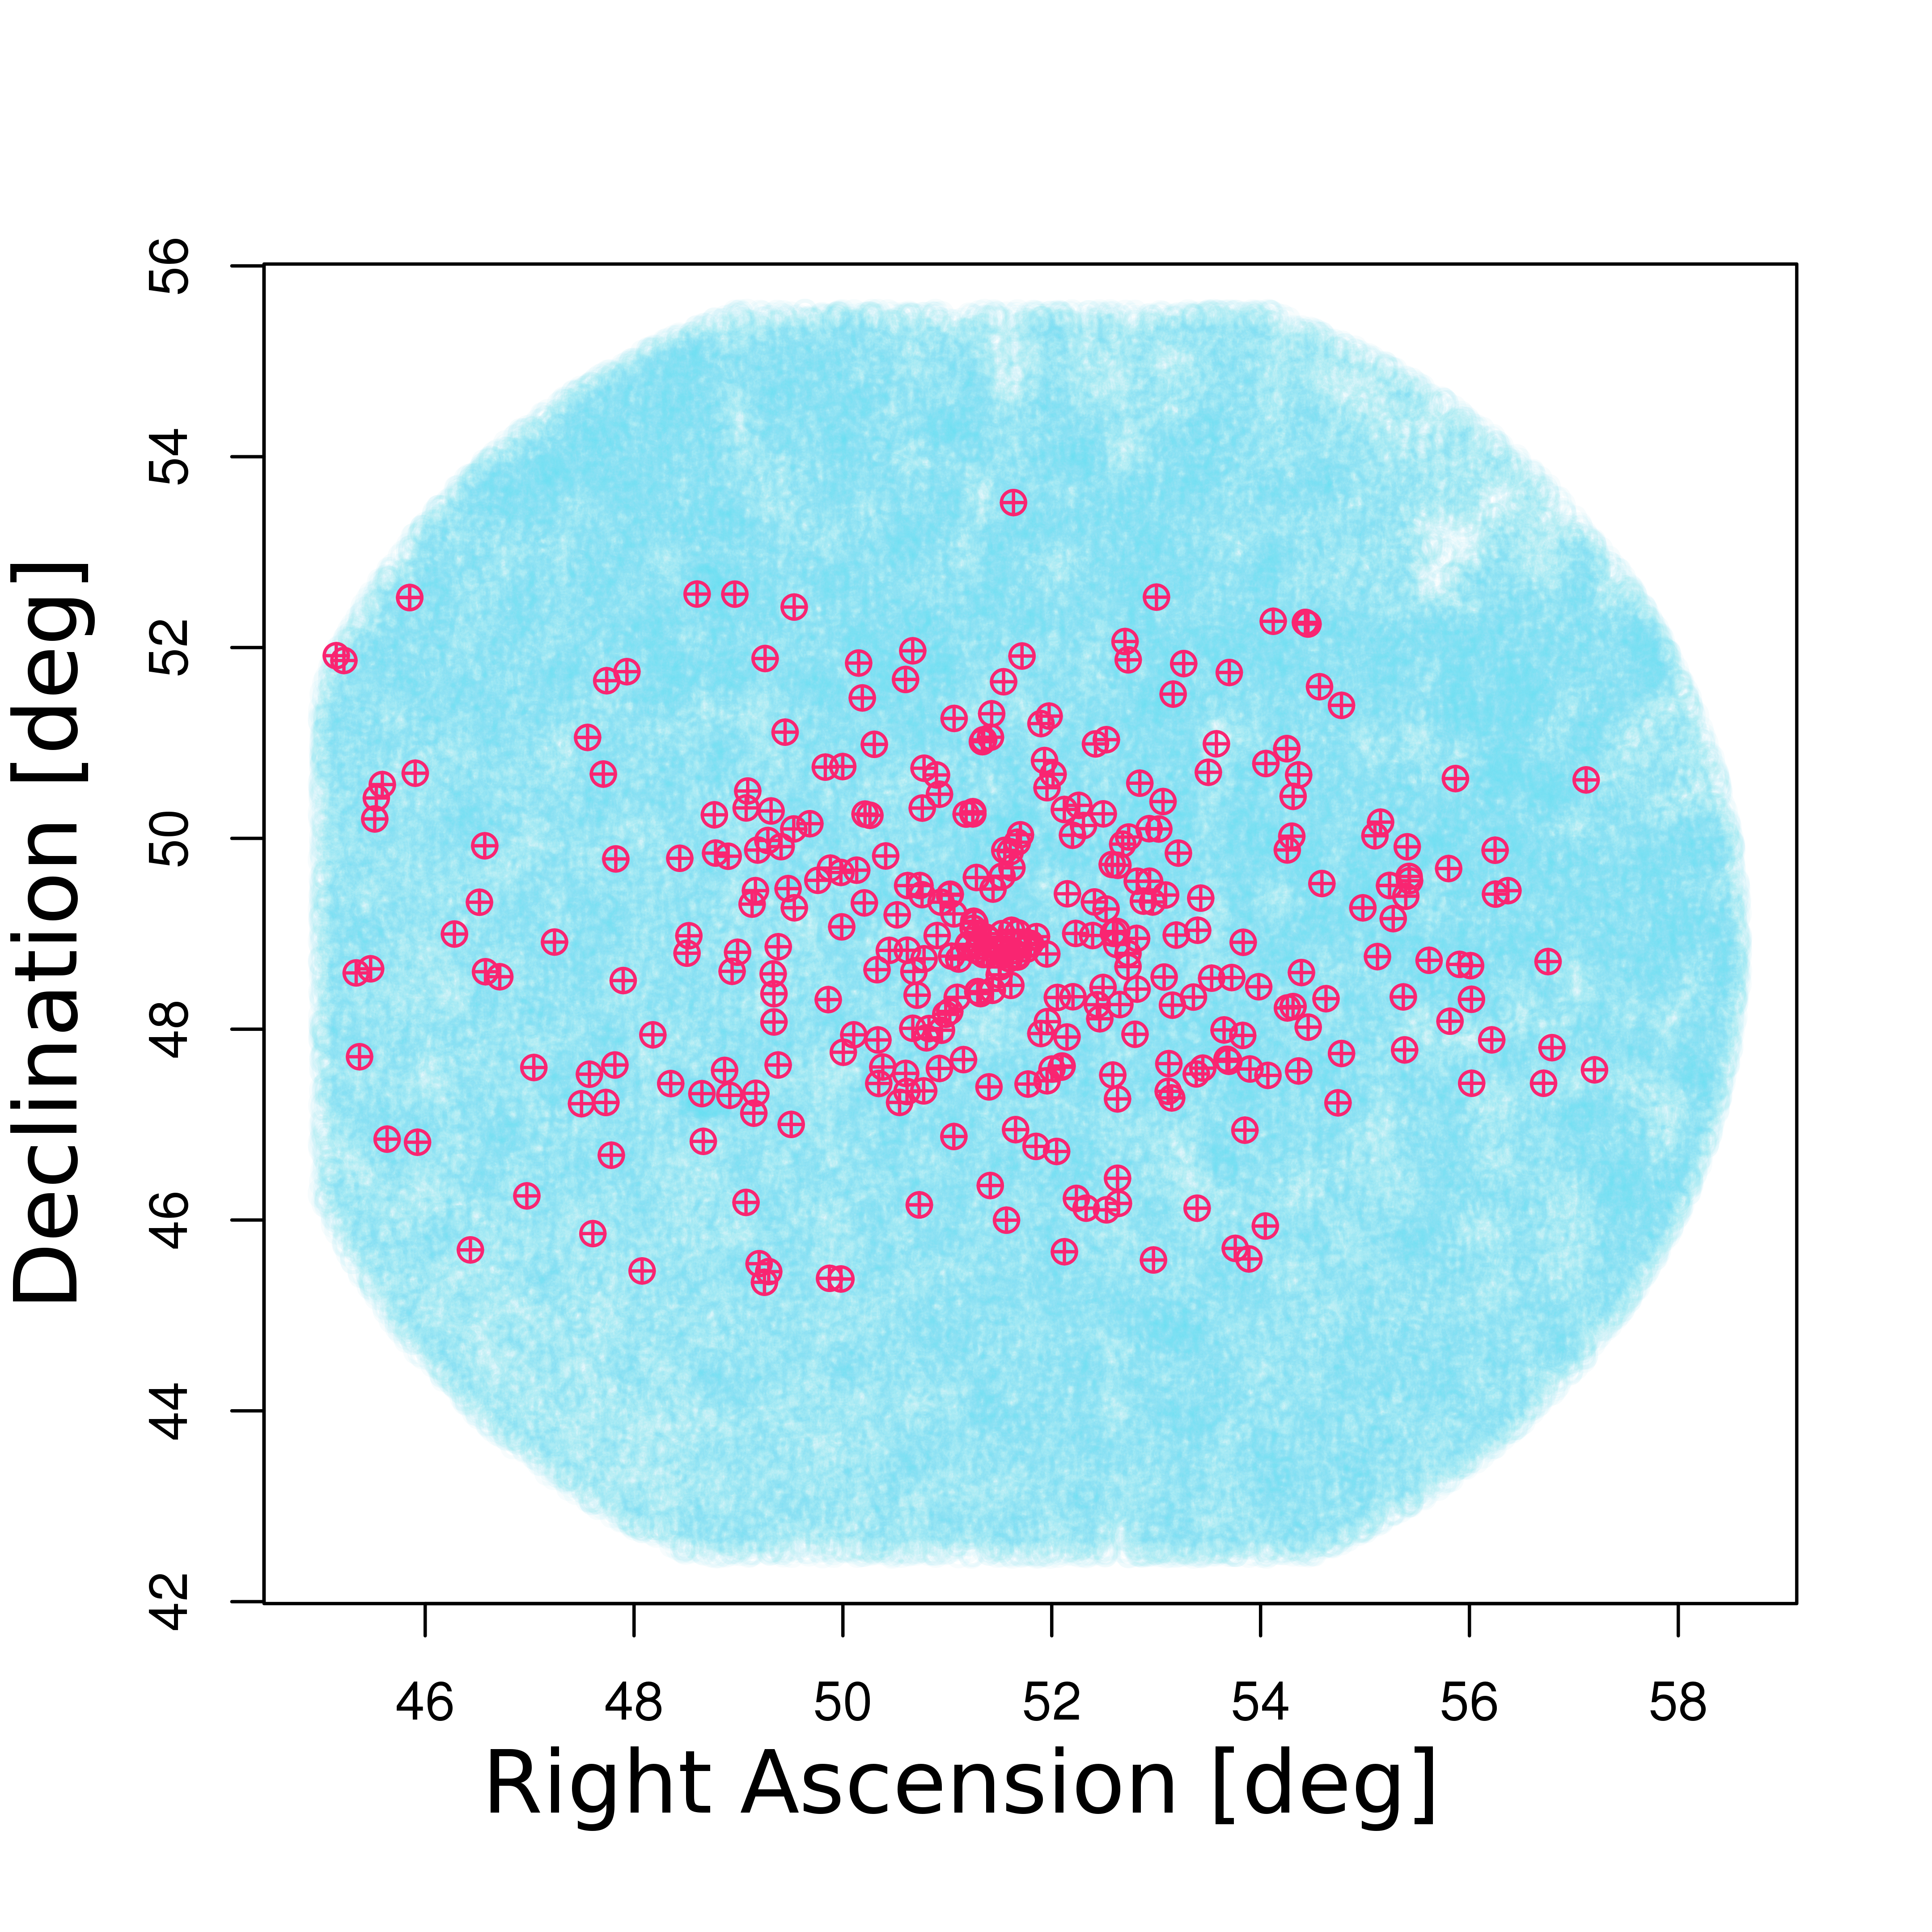
\includegraphics[scale=.9]{SpaDis2}
%\end{center}
%\end{tikzfigure}
%}
%\block[bodywidthscale=1.2,bodyoffsetx=.3in,titleoffsetx=.225in, bodyoffsety=1in, titleoffsety=.5in]{Proper Motion Distribution}{
%\begin{tikzfigure}[distribution in proper motion right ascension and proper motion declination. Member stars heavily localized, while field stars heavily localized elsewhere]
%\label{Fig. 4}
%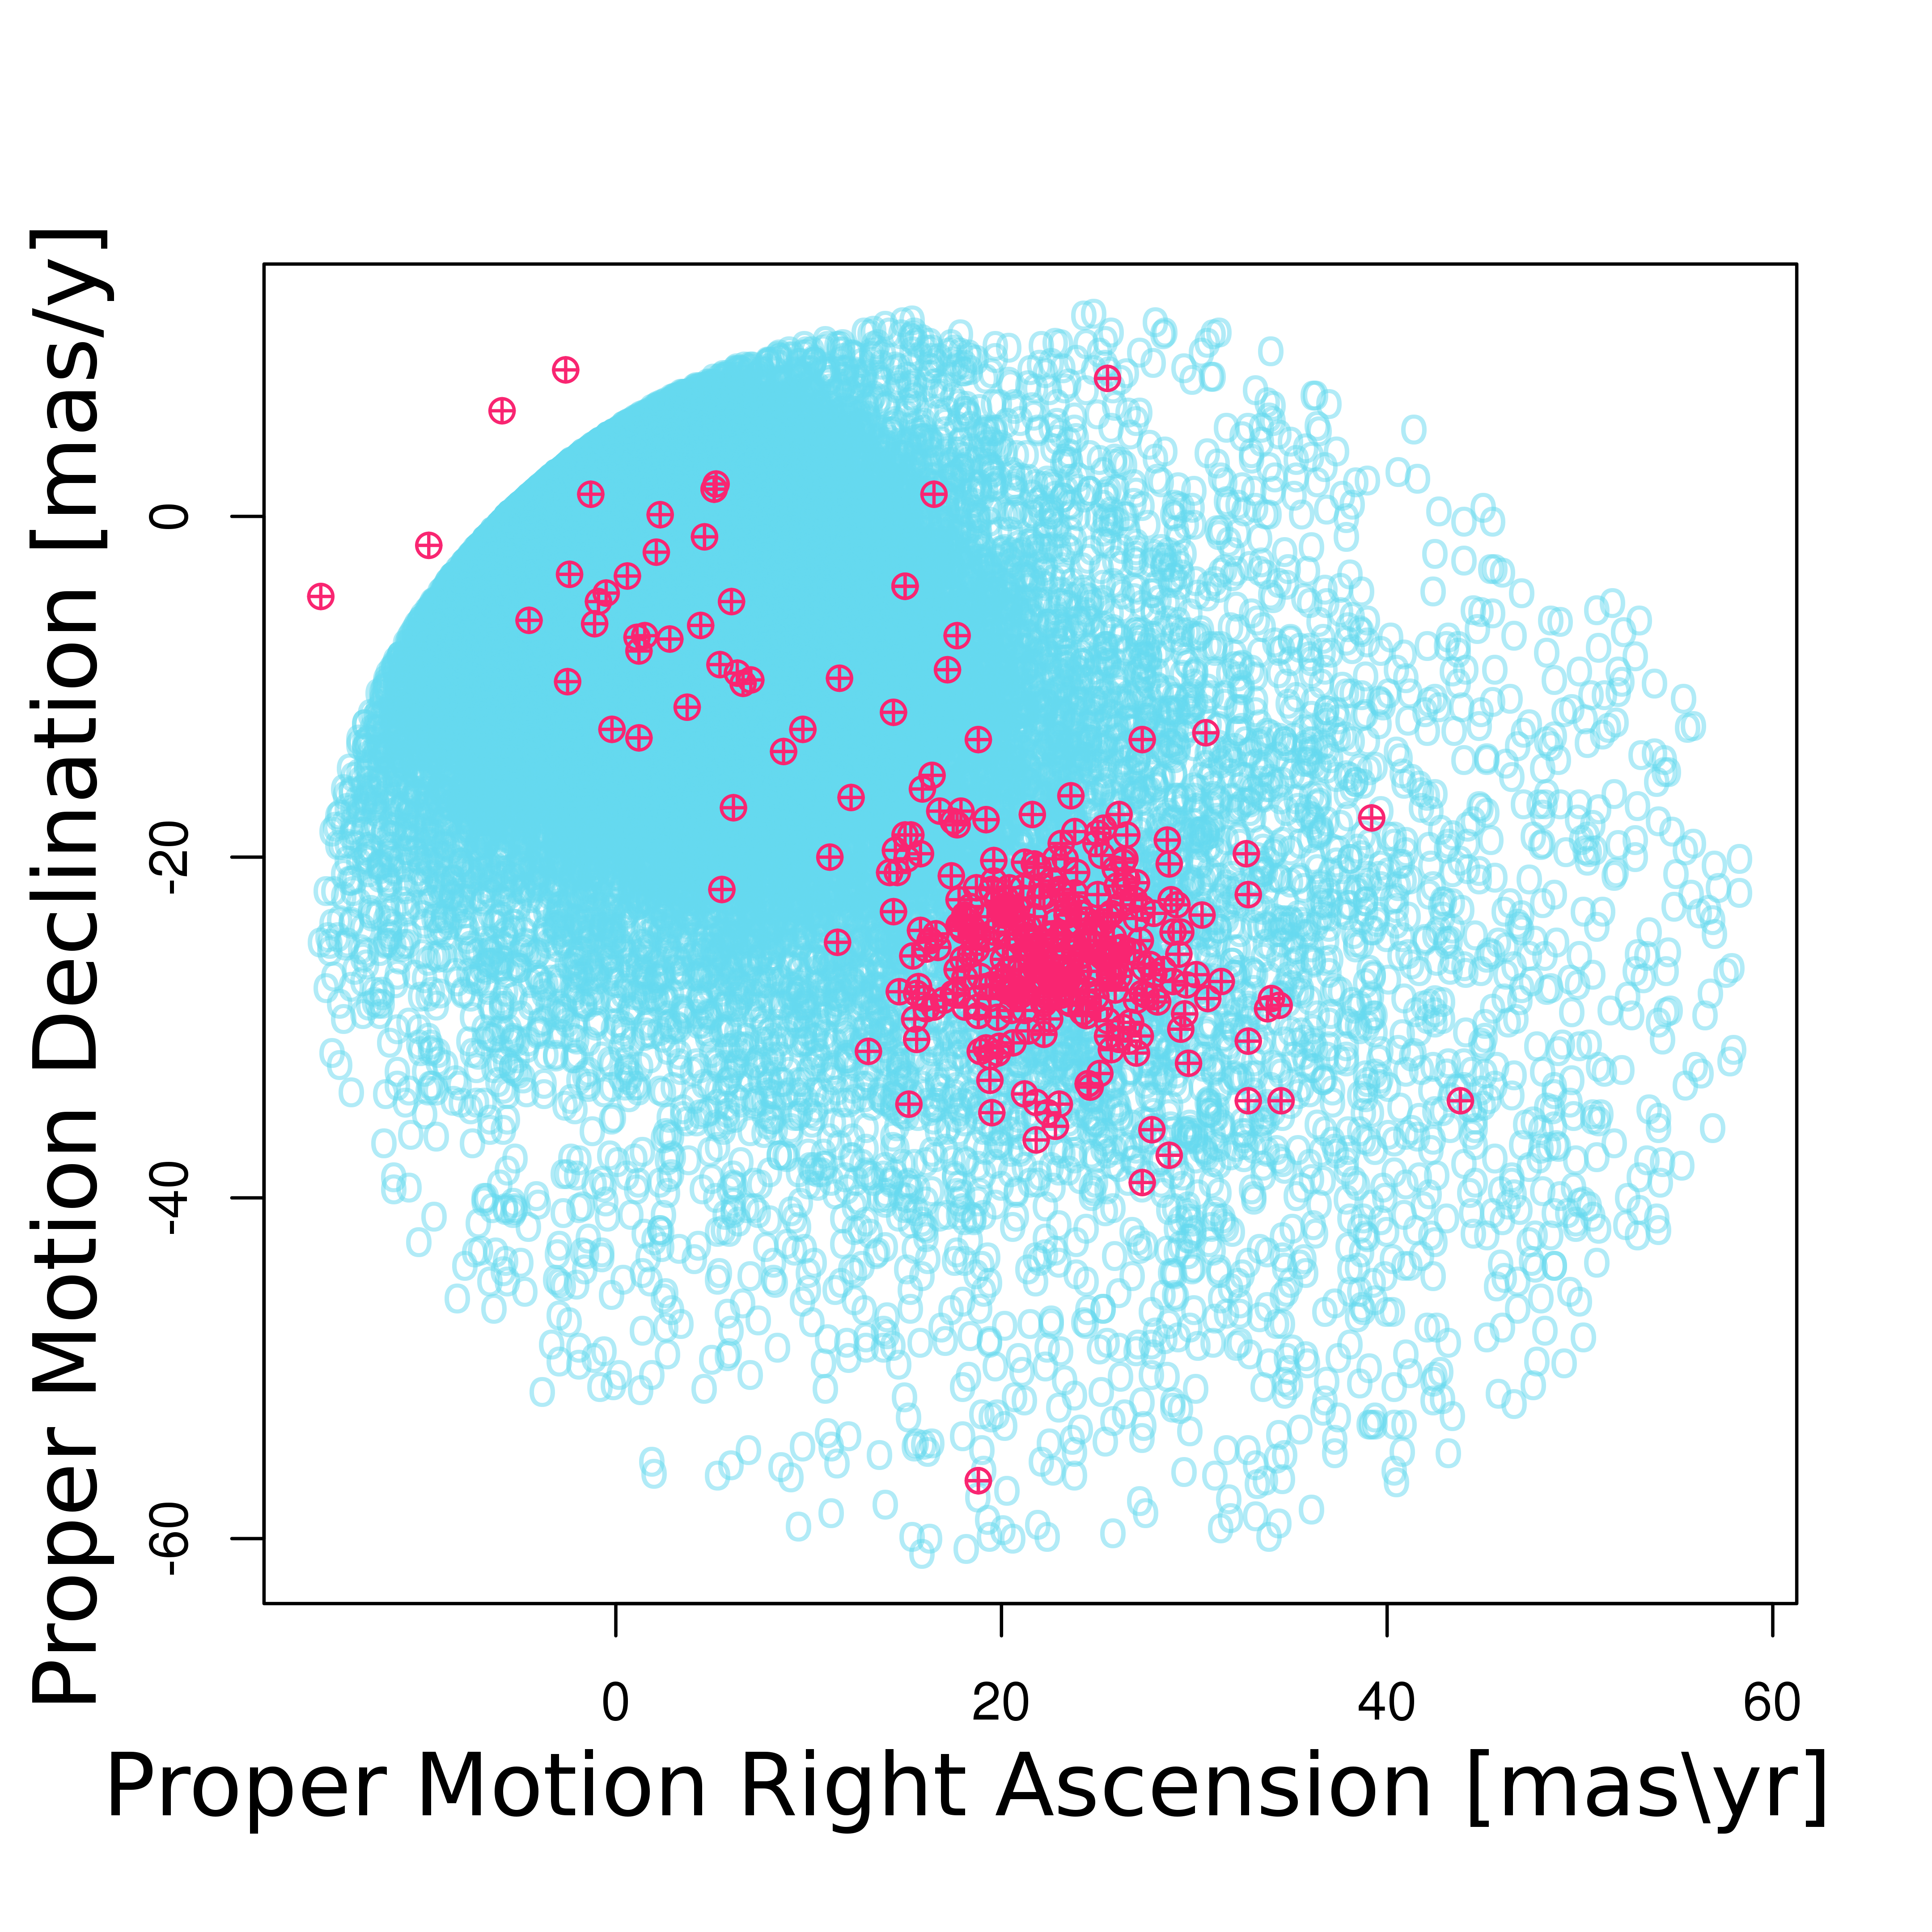
\includegraphics[scale=.9]{ProDis}
%\end{center}
%\end{tikzfigure}

%}
%\subcolumn{.45}
%\block[bodywidthscale=1.2,bodyoffsetx=.6in,titleoffsetx=.45in,bodyoffsety=1.69in, titleoffsety=.5in]{Spatial Probability}{
%\begin{tikzfigure}[Membership Probability over radial distance. Members show high probability at their distances relative to the catalog stars, due to high proper motion probability.]
%\label{Fig. 4}
%\includegraphics[scale=.9]{SpaPro}
%\end{tikzfigure}

%}
%\block[bodywidthscale=1.2,bodyoffsetx=.6in,titleoffsetx=.45in,bodyoffsety=1.71in,titleoffsety=.5in]{Proper Motion Probability}{
%\begin{tikzfigure}[Membership Probability over proper motion distance.  Member stars localized at low differences from the mean proper motion.]
%\label{Fig. 5}
%\includegraphics[scale=.9]{ProPro}
%\end{tikzfigure}
%}
\end{columns}
%\Huge{\textbf{Membership Survey of the Alpha Persei Open Stellar Cluster}}\\
%\floatstyle{boxed}{\fbox{\includegraphics{poster3dalpha}}}\hspace{2.75in}\floatstyle{boxed}{\fbox{\includegraphics{abstract}}}
%\begin{comment}
%\includegraphics{plot3dalpha}\includegraphics{abstract}
%\center{\floatstyle{boxed}{\fbox{\includegraphics{desc}}}}
%\floatstyle{boxed}{\fbox{\includegraphics{SpaDis}}}\hspace{2.75in}\floatstyle{boxed}{\fbox{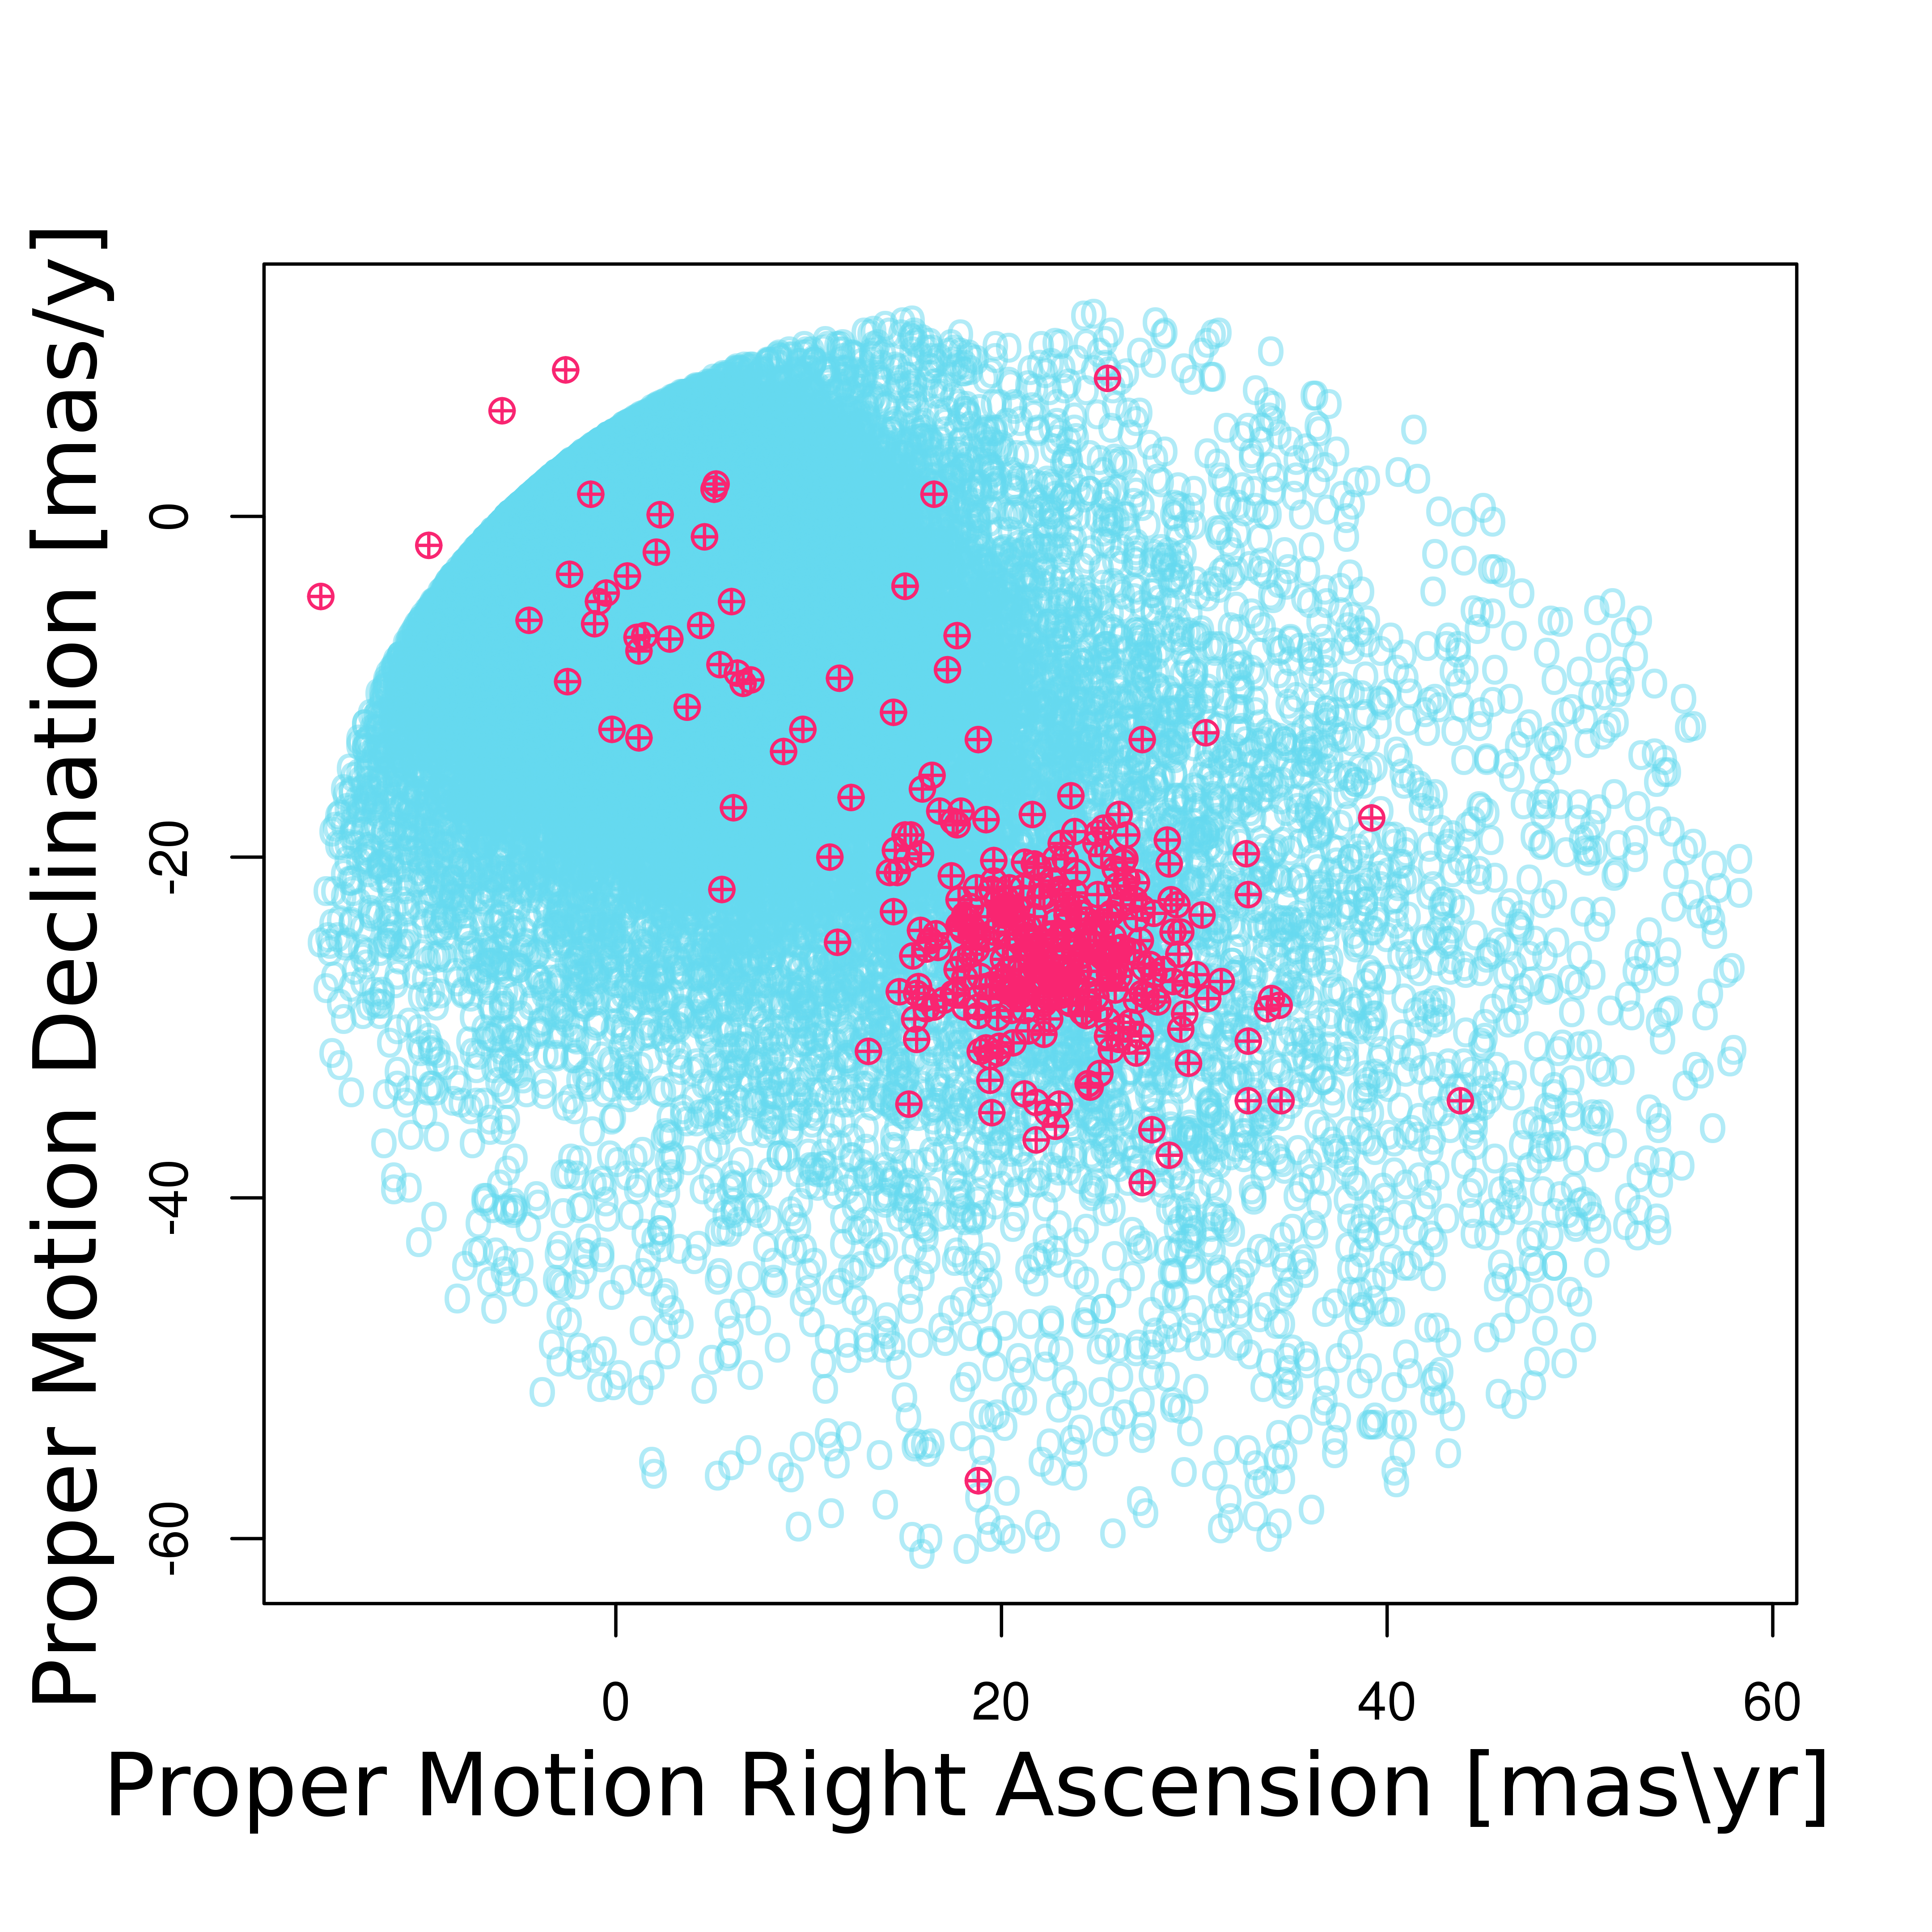
\includegraphics{ProDis}}}
%\begin{tabular}{@{}c@{} @{}c@{}}
%\includegraphics{mehtods2}&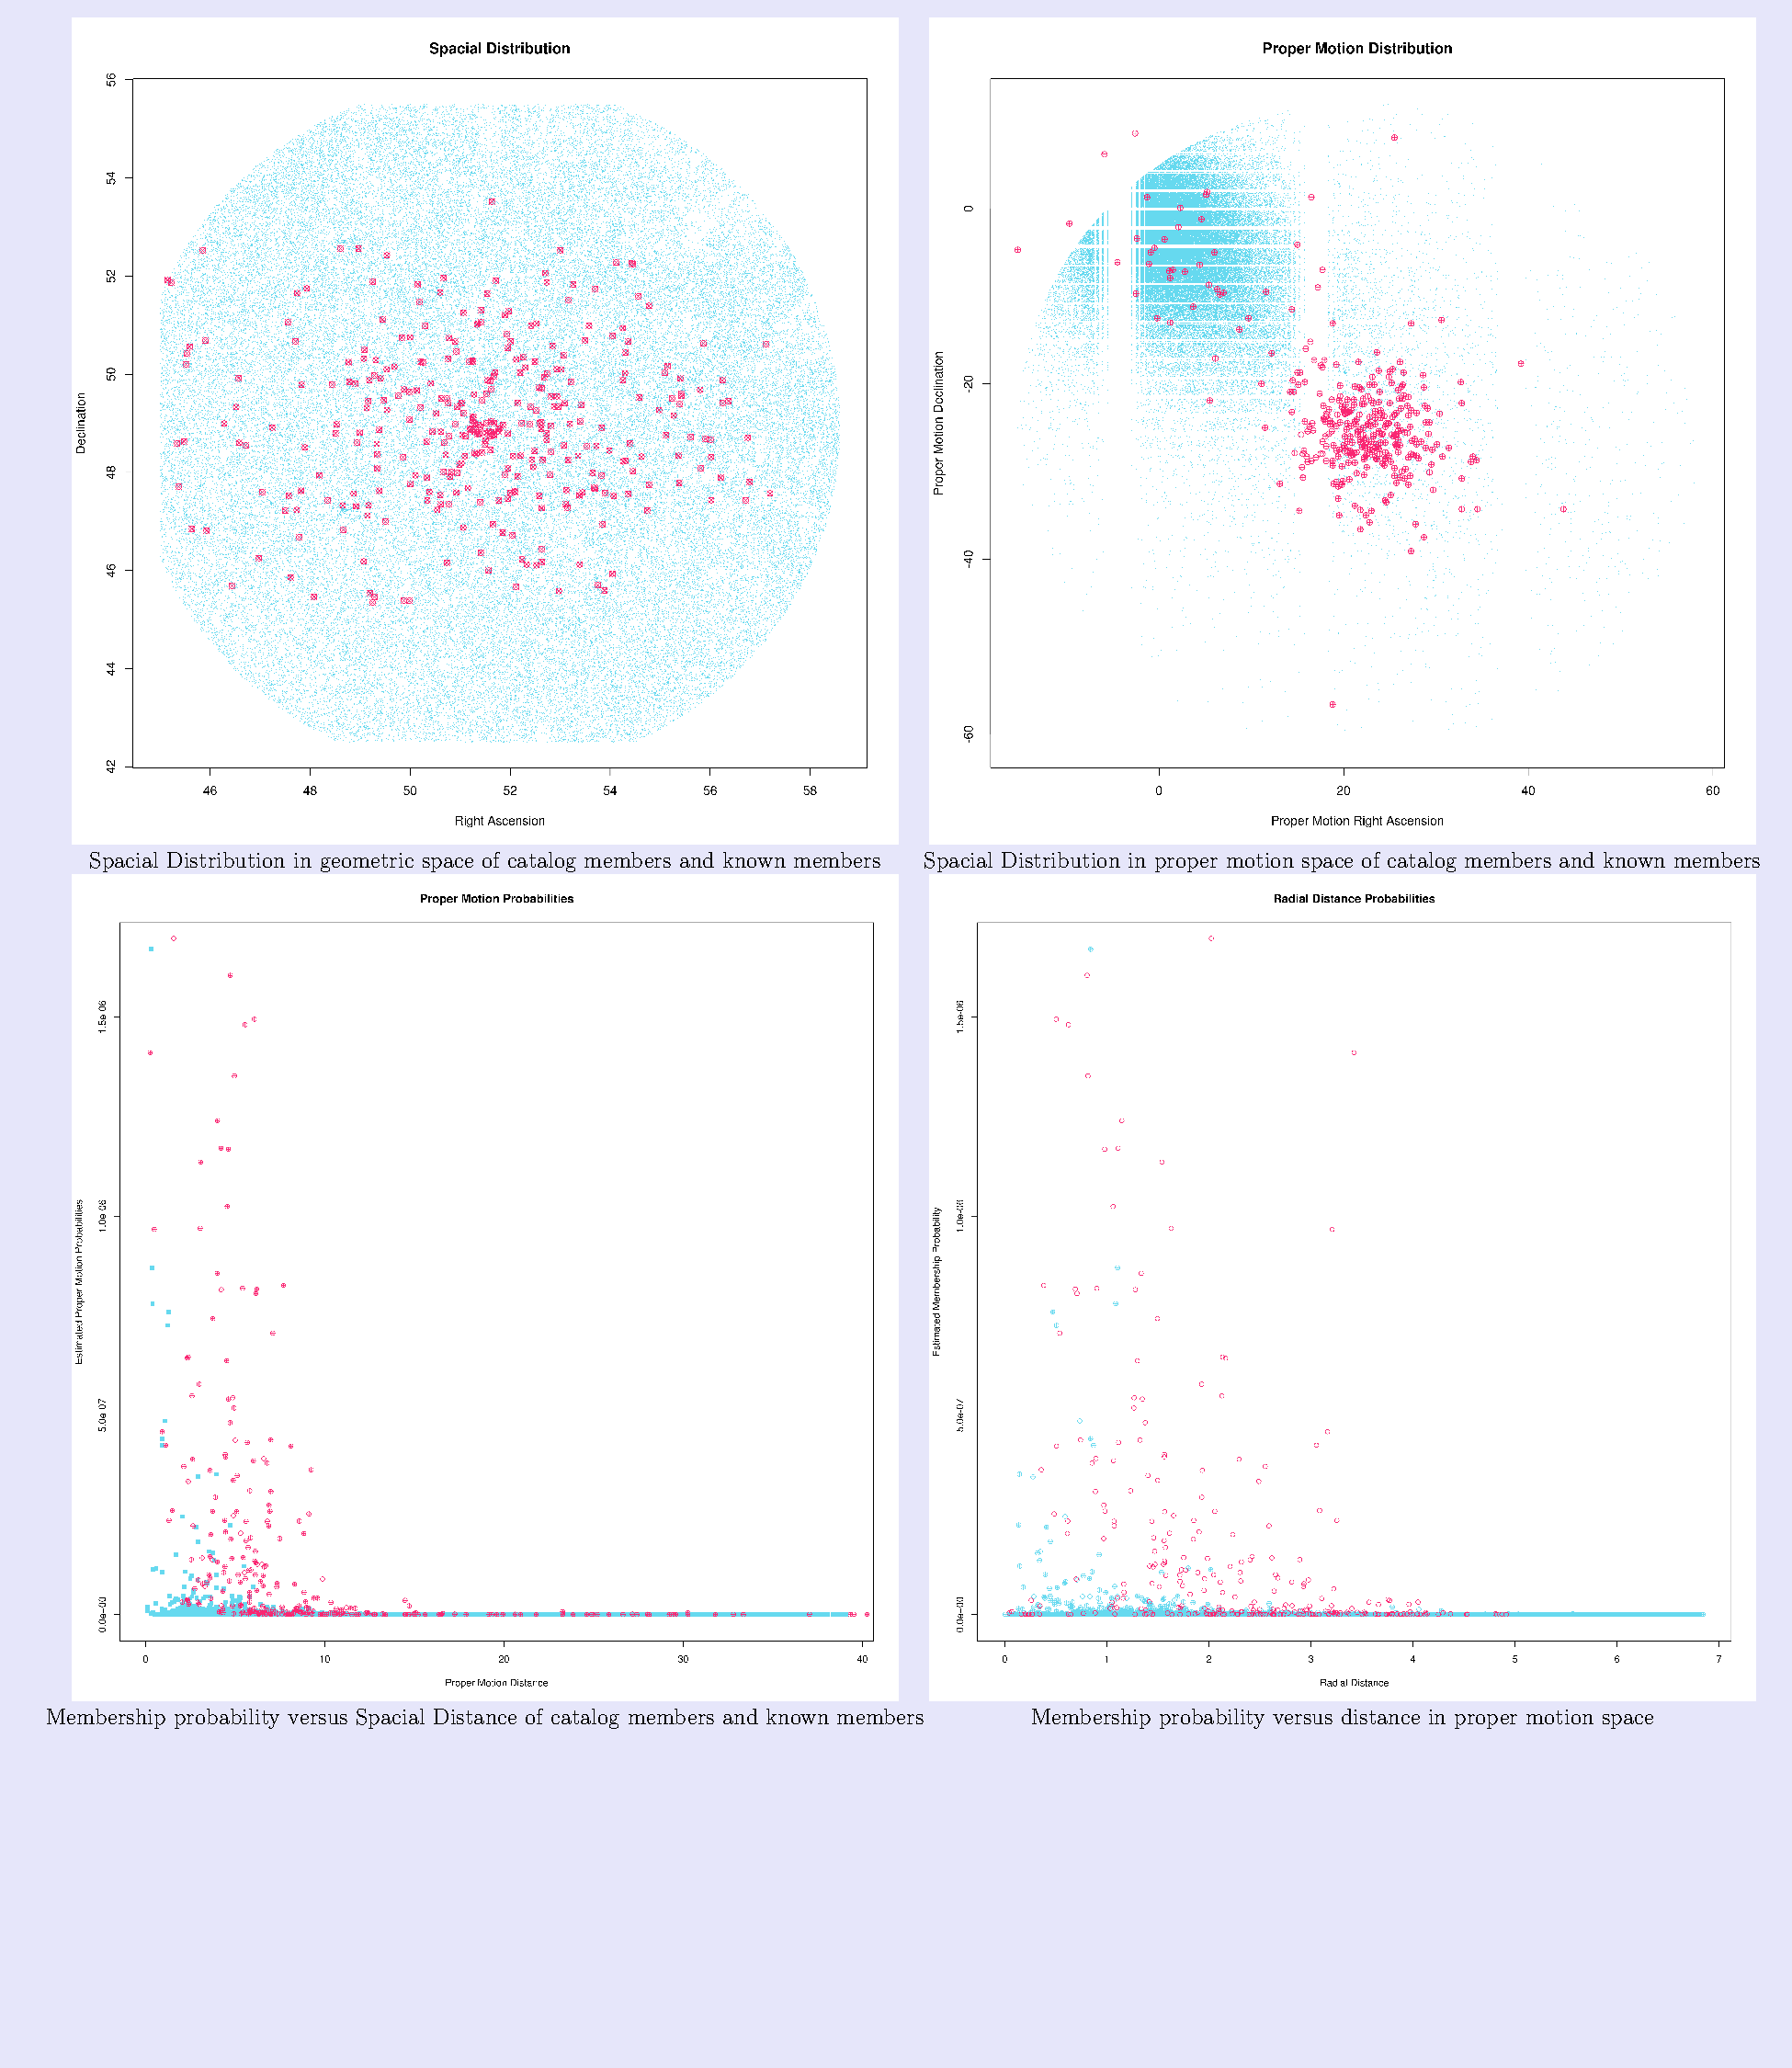
\includegraphics{fourgraphs}
%\end{tabular}
%\end{comment}
\end{centering}
\end{document}
